% ----------------------------------------------------------------
%% Thesis.tex -- MAIN FILE (the one that you compile with LaTeX)
%% ---------------------------------------------------------------- 

% Set up the document
\documentclass[a4paper, 11pt, oneside]{Thesis}  % Use the "Thesis" style, based on the ECS Thesis style by Steve Gunn
%\graphicspath{Figures/}  % Location of the graphics files (set up for graphics to be in PDF format)
\usepackage{fancyhdr}
% Include any extra LaTeX packages required
\usepackage[square, numbers, comma, sort&compress]{natbib}  % Use the "Natbib" style for the references in the Bibliography
\usepackage{verbatim}  % Needed for the "comment" environment to make LaTeX comments
\usepackage{vector}  % Allows "\bvec{}" and "\buvec{}" for "blackboard" style bold vectors in maths
\usepackage{graphicx} 
\hypersetup{urlcolor=blue, colorlinks=true}  % Colours hyperlinks in blue, but this can be distracting if there are many links.
%
\pagestyle{fancy}
\fancyhf{}  % Alle Kopfzeilen löschen
%% ----------------------------------------------------------------
\begin{document}
\begin{titlepage}

\newcommand{\HRule}{\rule{\linewidth}{0.5mm}} % Defines a new command for the horizontal lines, change thickness here

\center % Center everything on the page
 %----------------------------------------------------------------------------------------
%	LOGO SECTION
%----------------------------------------------------------------------------------------
\begin{minipage}{0.4\textwidth}
\begin{flushleft} \large

\includegraphics[width=5cm, height=1.2cm]{Pictures/UST.jpg}
\end{flushleft}
\end{minipage}

\begin{minipage}{0.4\textwidth}
\begin{flushright} \large

\includegraphics[width=5cm, height=1.2cm]{Pictures/ILH.jpg}
\end{flushright}
\end{minipage}\\[2cm]
 % Include a department/university logo - this will require the graphicx package
%----------------------------------------------------------------------------------------
%	HEADING SECTIONS
%----------------------------------------------------------------------------------------

\textsc{\LARGE \bfseries Fachpraktikum (Bachelor)}\\[0.2cm] % Name of your university/college
\textsc{\LARGE 6G Hardwarelabor - Design und Implementierung eines HF Transceivers}\\[0.2cm] 
%\textsc{\LARGE Design}\\[0.5cm] 
%\textsc{\Large ILH}\\[0.5cm] % Major heading such as course name
%\textsc{\large PuL-Analog Microwave Frontend Design}\\[0.5cm] % Minor heading such as course title

%----------------------------------------------------------------------------------------
%	TITLE SECTION
%----------------------------------------------------------------------------------------

\HRule \\[0.4cm]
{ \huge \bfseries Versuch 1: Drahtlose Übertragungen und Link-Budget}\\[0.4cm] % Title of your document
\HRule \\[1.5cm]
 
%----------------------------------------------------------------------------------------
%	AUTHOR SECTION
%----------------------------------------------------------------------------------------
\textbf{Protokollführer}\\
{\large\ Lukas Müller}\\[0.5cm]
\textbf{Versuchspartner}\\
{\large\ Andric Steiner}\\[0.2cm]
{\large\ Erik Zimmerman}\\[0.2cm]
{\large\ Farhad Valizada}\\[0.2cm]
{\large\ Samuel Brunner}\\[0.2cm]
{\large\ Tari Kausler}\\[0.7cm]

\textbf{Betreuer}\\
{\large\ Simon Haussmann}\\[0.2cm]



%----------------------------------------------------------------------------------------
%	DATE SECTION
%----------------------------------------------------------------------------------------
\textbf{Eingereicht}\\
{\large \today} % Date, change the \today to a set date if you want to be precise

 
%----------------------------------------------------------------------------------------

\vfill % Fill the rest of the page with whitespace

\end{titlepage}


%\vfill\vfill\vfill\vfill\vfill\vfill\null
\clearpage  % Funny Quote page ended, start a new page
%% ----------------------------------------------------------------

% The Abstract Page


%% ----------------------------------------------------------------

\setstretch{1.3}  % Reset the line-spacing to 1.3 for body text (if it has changed)

% The Acknowledgements page, for thanking everyone
%\acknowledgements{
%\addtocontents{toc}{\vspace{1em}}  % Add a gap in the Contents, for aesthetics
%
%The acknowledgements and the people to thank go here, don't forget to include your project advisor\ldots
%
%}
%\clearpage  % End of the Acknowledgements1
%% ----------------------------------------------------------------

%\pagestyle{fancy}  %The page style headers have been "empty" all this time, now use the "fancy" headers as defined before to bring them back




\renewcommand{\contentsname}{Inhaltsverzeichnis}
\tableofcontents
\newpage

\chapter{Einleitung}
\section{Relevanz der Funkübertragung im Alltag}
Jeden Tag nutzen wir Funkübertragungen in verschiedenen Formen, sei es durch WLAN, Bluetooth oder Mobilfunk. Diese Technologien ermöglichen es uns, Daten über große Entfernungen zu übertragen, ohne physische Verbindungen herstellen zu müssen. Die Grundlagen der Modulation sind entscheidend für die Entwicklung und Verbesserung dieser Technologien.
Die \ac{6G} der Funkübertragung ist die neueste Generation der Funkkommunikation, die eine höhere Datenrate, geringere Latenz und verbesserte Zuverlässigkeit verspricht. Sie ist aktuell in der Entwicklung, 
jedoch besteht bei dem Frequenzbereich von \ac{6G}, beginnend mit Sub-6 GHz (unter 6 GHz) bis hin zu THz-Bereich (100 GHz - 1 THz), 
die Herausforderung, dass die Signale bei höheren Frequenzen stärker gedämpft werden und somit eine höhere Signalstärke erforderlich ist, um eine zuverlässige Kommunikation zu gewährleisten.
Deswegen ist es leichter, eine beispielhafte Funkübertragung bei kleineren Abständen zu dimensionieren, um das Wissen bei größeren Strecken anwenden zu können.
\section{Ziel des Versuchs}
Das Ziel des heutigen und des letzten Versuchs ist es, eine Bildübertragung über eine Funkverbindung zu realisieren und dabei die Grundlagen der Bildübertragung mithilfe von 6G zu verstehen.
Dies bietet einen guten Einblick in die digitale Kommunikation und die Modulation von Signalen, die für die Übertragung von Daten über Funkverbindungen unerlässlich ist.
\clearpage 

\chapter{Theoretische Grundlagen}
\section{Modulationsarten}

\section{Blockdiagramm einer Sendestrecke}
\subsection{DAC}
\subsection{LO}
\subsection{Mischer} 
\subsection{PA}
\subsection{Antennen}
\subsection{LNA}
\subsection{Demodulation}
\subsection{ADC}
\section{Mathematische Grundlagen: Fourier-Transformation}
\subsection{Betrag und zeitlicher Verlauf von Rechteckfunktion}
\subsection{Betrag und zeitlicher Verlauf von Sinusfunktion}
\subsection{Multiplikation der beiden Funktionen im Zeitbereich}
\section{Zusammenhang von Datenrate und Bandbreite}
blabla
\clearpage


\chapter{Versuchsaufbau}

\section{Verwendete Geräte}
In diesem Versuch wurden folgende Geräte verwendet:
\begin{itemize}
    \item \textbf{Keysight Fieldfox Network Analyzer N9918A}: Zur Messung der S-Parameter des Filters.
    \item \textbf{Signal Generator}: Zur Erzeugung eines Testsignals, das durch den Filter geleitet wird.
    \item \textbf{Coupled-Line-Filter}: Das zu messende Filter, das in ADS entworfen und simuliert wurde. (siehe Schaltplan\_PCB\_V4)
\end{itemize}
\clearpage

\chapter{Durchführung}

\section{Task 1: Kabel charakterisieren}
\section{Task 2: Ausgangsleistung messen}
\section{Task 3: Fundamentalen Ton vermessen}
\section{Task 4: Funkübertragungsexperiment}
\section{Task 5: Link Budget berechnen}
blabla
\clearpage

\chapter{Ergebnisse}


\section{Tabellen und Diagramme}
bla bla
\clearpage

\chapter{Diskussion}
\section{Vergleich von Theorie und Praxis}
\section{Erklärung von Abweichungen}
bla bla
\clearpage

\chapter{Fazit}

Im Verlauf dieses Versuches konnten wir die grundlegende Funktionsweise eines Coupled Line Filters praktisch nachvollziehen und ebenfalls unser theoretisches Wissen erweitern. Es ist sehr interessant zu sehen, wie sich die anfangs unscheinbaren Platine zu einem komplexen Konstrukt entwickelt deren einzelnen Komponenten und deren Zusammenspiel wir nach und nach immer besser verstehen. Ebenfalls ist die Arbeit mit der Simmulationssofware ADS äußerst erkenntnisreich und hilft uns die Fehler in dem praktischen Teil des Versuches zu identifizieren und zu sehen, wie es unter optimalen Bedingungen aussehen müsste. Es gibt noch vieles zu lernen im Verlauf dieses Praktikums und wir sind gespannt auf das was noch kommt. 
\clearpage  

\chapter{Literaturverzeichnis}
\begin{thebibliography}{1}
\bibitem{infineon_lna}
Infineon Technologies AG: \emph{BFR181W Silicon NPN RF Transistor}, Datenblatt, 2017. Online verfügbar unter: \url{https://www.infineon.com/dgdl/Infineon-BFR181W-DS-v02_00-en.pdf}
\end{thebibliography}
%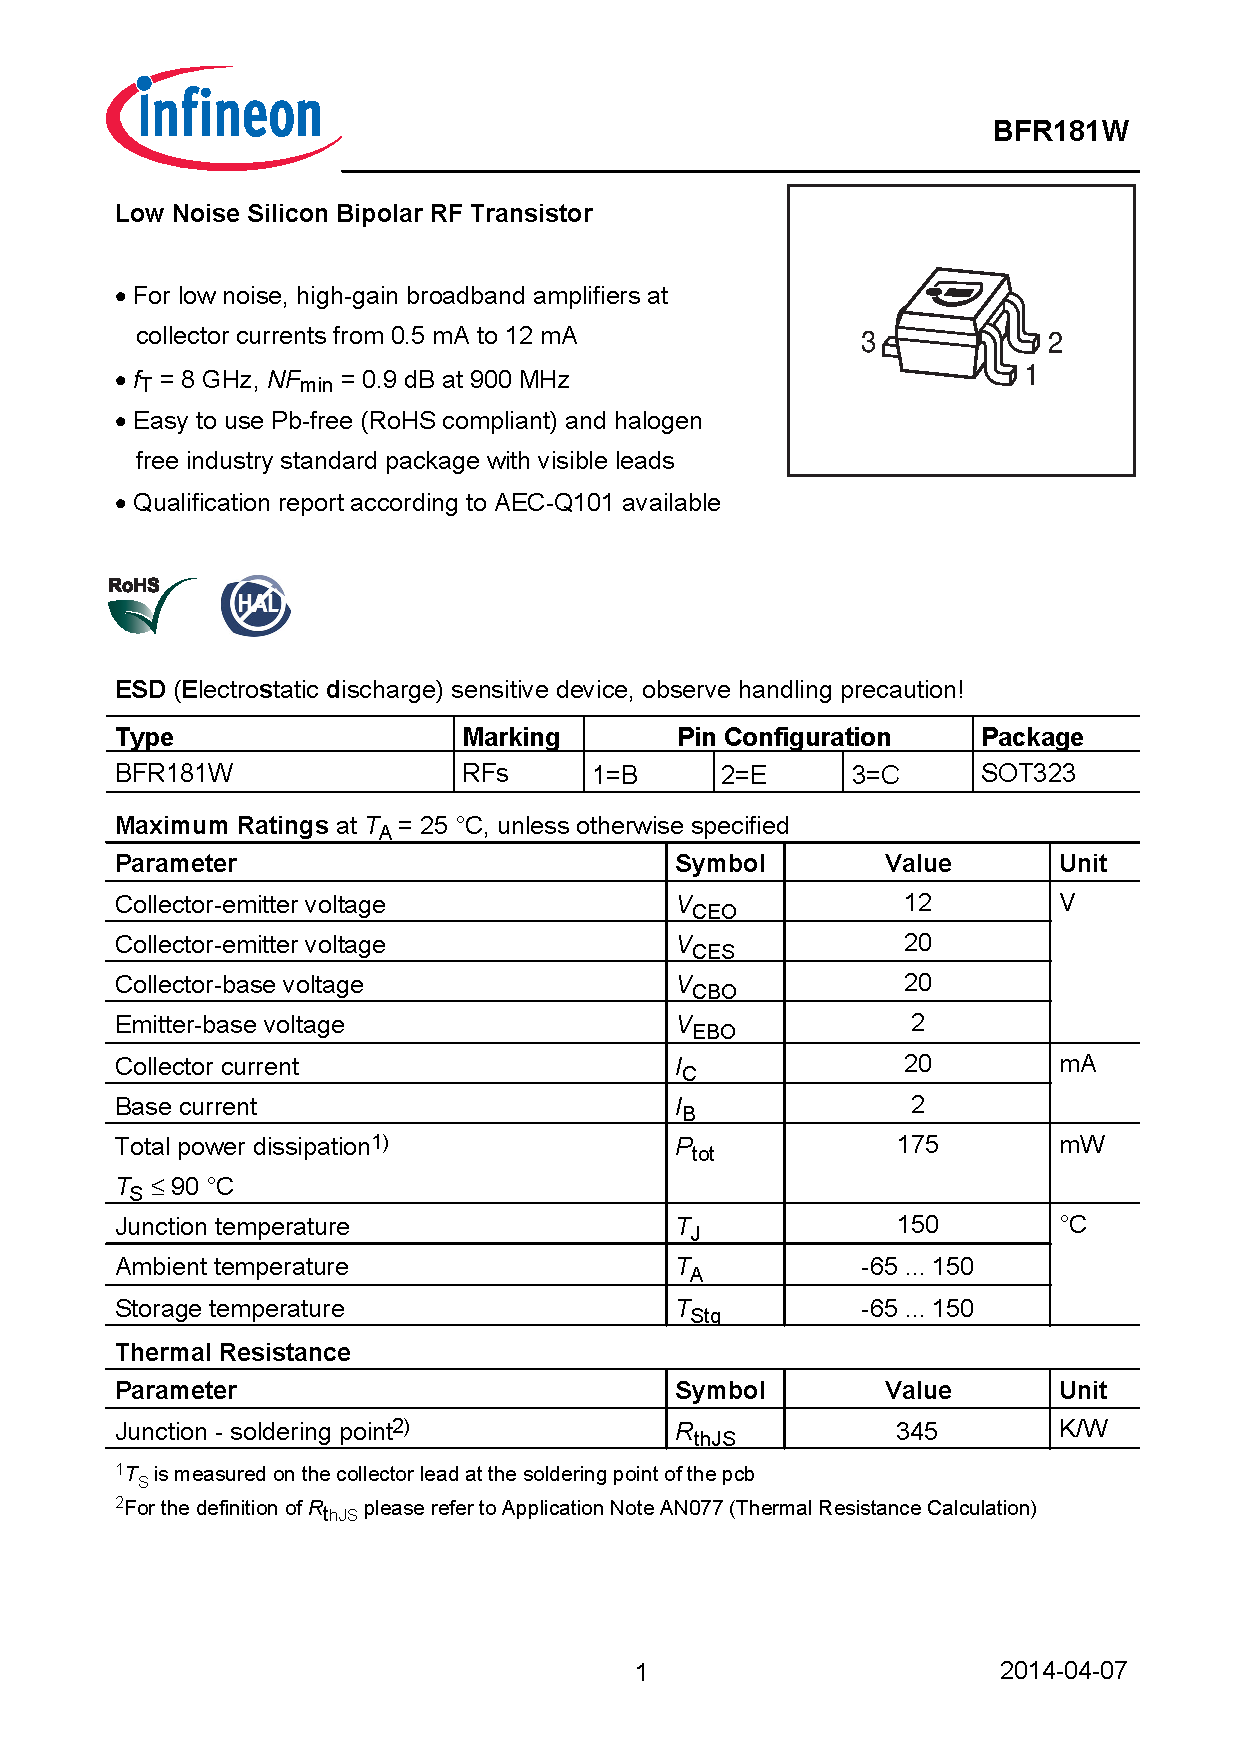
\includepdf[pages=-, pagecommand={\thispagestyle{empty}\setcounter{page}{\thepage}\rfoot{\thepage}}, fitpaper=true, offset=1.0in -1.0in]{C:/Users/Farhad/OneDrive/Desktop/Vorlage neu/GrundlagenPraktikum6G/2_Protokoll/Literature/Infineon_LNA_BFR181W-85922.pdf}
\clearpage

\chapter{tasks}
advanced Design System 2024
\section{task2:}
kollektor strom maximal  IC = 1.5mA

$I_CMax = 1.5mA$

\section{task3:}
um die BE FLuss spannung zu erreichefn
muss R3 auf exax
$R3 = 1950\Omega$\\
Nach der E12 Reihe entspricht $R3 = 2.2k\Omega$
\subsection{a}
berrechnen des kollektorwiderstanddes
\begin{equation}
    R_5 = \frac{U_{CC}}{I_CMax*0.75} = \frac{4.8V}{20mA *0.75}\Omega=320\Omega
    \\wegen E12 Reihe
     R_5 = 330\Omega
\end{equation}








\end{document}  % The End
%% ----------------------------------------------------------------